\documentclass[tikz,border=10pt]{standalone}
\begin{document}
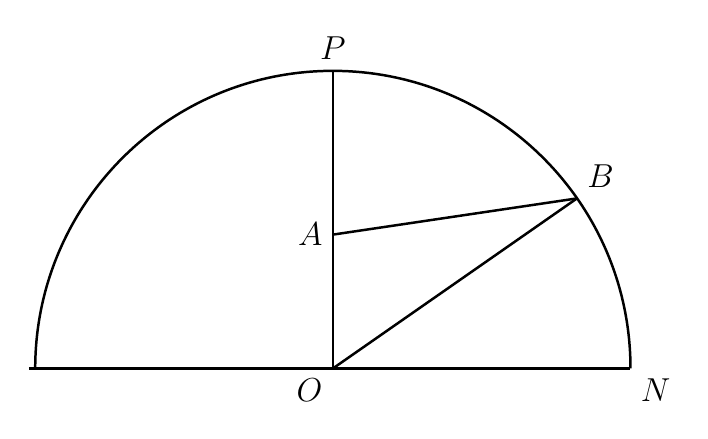
\begin{tikzpicture}[line join=round, line width=0.9pt]
% named coordinates (scale s = 0.016064 cm/px, y flipped, origin at O)
\coordinate (L) at (-3.86,0);     % left diameter end (unlabeled)
\coordinate (O) at (0,0);         % centre
\coordinate (N) at (3.78,0);      % right diameter end
\coordinate (P) at (0,3.79);      % top of semicircle
\coordinate (A) at (0,1.70);      % on segment OP
\coordinate (B) at (3.10,2.16);   % on arc

% diameter and upper semicircle (radius about 3.78 cm)
\draw (L) -- (N);
\draw (N) arc[start angle=0, end angle=180, radius=3.78];

% segments
\draw (O) -- (P);
\draw (A) -- (B);
\draw (O) -- (B);

% labels
\node[above, font=\fontsize{12.5}{15}\selectfont] at (P) {$P$};
\node[left, font=\fontsize{12.5}{15}\selectfont] at (A) {$A$};
\node[above right, font=\fontsize{12.5}{15}\selectfont] at (B) {$B$};
\node[below left, font=\fontsize{12.5}{15}\selectfont] at (O) {$O$};
\node[below right, font=\fontsize{12.5}{15}\selectfont] at (N) {$N$};
\end{tikzpicture}
\end{document}